\immediate\write18{makeindex -s nomencl.ist -o Management.nls Management.nlo}

%Layout packages
\documentclass[12pt]{article}
\usepackage[english]{babel}
\usepackage[utf8x]{inputenc}
\usepackage[letterpaper, margin=1.5in,margin=1.2in]{geometry}
\usepackage[colorinlistoftodos]{todonotes}

%Math
\usepackage{amsmath}

%Drawing
\usepackage{graphicx}
\usepackage{tikz}
\usetikzlibrary{shadows,arrows}
% Define the layers to draw the diagram
\pgfdeclarelayer{background}
\pgfdeclarelayer{foreground}
\pgfsetlayers{background,main,foreground}
 
% Define block styles  
\tikzstyle{texture}=[draw, fill=blue!20, text width=6.0em, text centered,
  minimum height=1.5em,drop shadow]
\tikzstyle{diagElt} = [texture, text width=8em, minimum width=10em,
  minimum height=3em, rounded corners, drop shadow]
\tikzstyle{texto} = [above, text width=6em, text centered]
\tikzstyle{linepart} = [draw, thick, color=black!50, -latex', dashed]
\tikzstyle{line} = [draw, thick, color=black!50, -latex']
\tikzstyle{ur}=[draw, text centered, minimum height=0.01em]
 
% Define distances for bordering
\newcommand{\blockdist}{1.3}
\newcommand{\edgedist}{1.5}

\newcommand{\diagElt}[3]{node (p#1) [diagElt]
  {#2\\{\scriptsize\textit{#3}}}}

% Draw background
\newcommand{\background}[5]{%
  \begin{pgfonlayer}{background}
    % Left-top corner of the background rectangle
    \path (#1.west |- #2.north)+(-1,0.6) node (a1) {};
    % Right-bottom corner of the background rectanle
    \path (#3.east |- #4.south)+(+0.6,-0.3) node (a2) {};
    % Draw the background
    \path[fill=yellow!20,rounded corners, draw=black!50, dashed]
      (a1) rectangle (a2);
    \path (a1.east |- a1.south)+(1,-0.35) node (u1)[texto]
      {\scriptsize\textit{#5}};
  \end{pgfonlayer}}

\newcommand{\interOutput}[3]{%
  \path [linepart] (#1.east) -- node [above]
    {\scriptsize interOutput #2} (#3);}

\newcommand{\illu}[3]{%
	\begin{figure}[ht!]
			  \centering
			  \includegraphics[scale=#3]{graphics/#1}
			  \caption{#2}
			  \smallskip
	\end{figure}}



\usepackage[refpage]{nomencl}
\makenomenclature

\begin{document}

\begin{titlepage}

\newcommand{\HRule}{\rule{\linewidth}{0.5mm}} % Defines a new command for the horizontal lines, change thickness here

\center % Center everything on the page
 
%----------------------------------------------------------------------------------------
%   HEADING SECTIONS
%----------------------------------------------------------------------------------------

\textsc{\LARGE University of Arizona}\\[1.5cm] % Name of your university/college
\textsc{\Large Mechatronics Class}\\[0.5cm] % Major heading such as course name
\textsc{\large Embedded Accelerometer Project}\\[0.5cm] % Minor heading such as course title

%----------------------------------------------------------------------------------------
%   TITLE SECTION
%----------------------------------------------------------------------------------------

\HRule \\[0.4cm]
{ \huge \bfseries Project Documentation}\\[0.4cm] % Title of your document
{ \Large \bfseries Project Management}\\[0.4cm] % Title of your document
\HRule \\[1.5cm]

%----------------------------------------------------------------------------------------
%   DATE SECTION
%----------------------------------------------------------------------------------------

{\large \today}\\[1.5cm] % Date, change the \today to a set date if you want to be precise

 
%----------------------------------------------------------------------------------------
%   AUTHOR SECTION
%----------------------------------------------------------------------------------------
\large\emph{Authors:}\\
Adrien \textsc{Bouskela}\small (adrien.bouskela@ipsa.fr)\\
Gregory \textsc{Largange}\small (gregory.largange@ipsa.fr)\\
Guillaume \textsc{Biton} \small (guillaume.biton@ipsa.fr)\\[1cm]

\large\emph{Mentors:}\\
Zoltan \textsc{Szabo}\small (zoltanszabo@email.arizona.edu)\\
\textsc{Dr. Enikov}\small (enikov@email.arizona.edu)\\[1.5cm]

%----------------------------------------------------------------------------------------
%   LOGO SECTION
%----------------------------------------------------------------------------------------

\includegraphics[scale=0.3]{Graphics/logo.png}\\[1cm] % Include a department/university logo - this will require the graphicx package
 
%----------------------------------------------------------------------------------------

\vfill % Fill the rest of the page with whitespace

\end{titlepage}

\newpage
\tableofcontents
\newpage

\section{Introduction}

	Shortly after being introduced to Mechatronics, we were assigned the following project. It was a challenging and motivating way to use our new skills in Mechatronics, but also a good project management training.\\
	The goal was to come up with a technical solution to reccord three-axis accelerations during a model rocket's flight and then recover them for "post-flight" analysis purpose.\\
	It has been decided that we would use a Microchip$^{\mbox{\scriptsize{\textregistered}}}$  microcontroller from PIC16F family (which we studied in Mechatronics class), a Serial EEPROM \nomenclature{EEPROM}{Electrically Erasable Programmable Read-Only Memory} module for data storage and an analog accelerometer as a sensor.\\
	The overall project was devided into subtasks, carried out by seven different teams. Our's was responsible for project management.\\
	Therefore, this document will especially deal with management issues while trying to provide an overlook of the project in its globality.\\
	Much of this document is about analizing our mistakes, explaining how we overcame difficulties and describe how we would do things if we had the opportunity of starting from scrach. We could probably encourage our readers who might be participating in a similar project to pay more attention to those post-analysis than to how we actualy did things.
\newpage
\section{Subdivision of the project}

	Starting with one specific goal, and knowing what exact resources we had (both human and material), our first step was logicly to decompose our main goal into subtasks to be able to allocate the workforce and tools.\\

	The basics of Mechatronics as well as common sense gave us the obvious scheme for our system:

	\begin{center}
	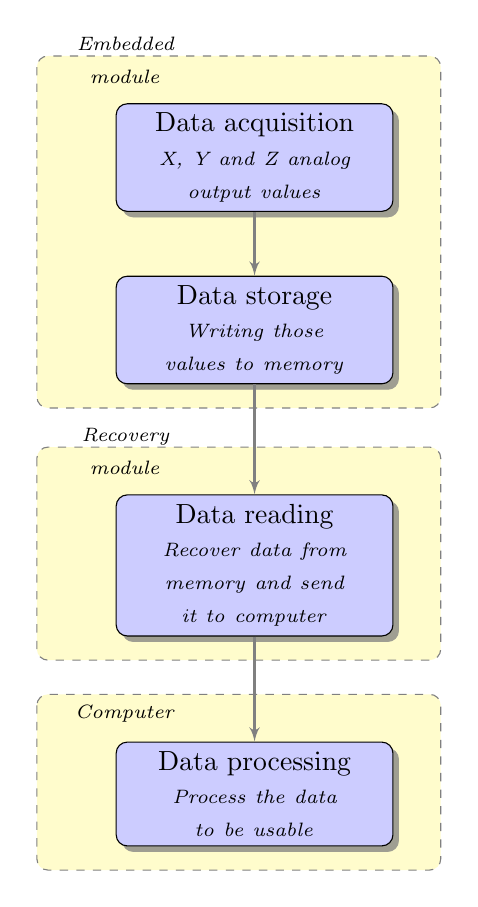
\begin{tikzpicture}[transform shape]
 
  % Draw diagram elements
  \path \diagElt {1}{Data acquisition}{X, Y and Z analog output values};
  \path (p1.south)+(0.0,-1.5) \diagElt{2}{Data storage}{Writing those values to memory};
  \path (p2.south)+(0.0,-2.3)  \diagElt{3}{Data reading}{Recover data from memory and send it to computer};
  \path (p3.south)+(0.0,-2.0) \diagElt{4}{Data processing}{Process the data to be usable};

 
  % Draw arrows between elements
  \path [line] (p1.south) -- node [above] {} (p2);
  \path [line] (p2.south) -- node [above] {} (p3);
  \path [line] (p3.south) -- node [above] {} (p4);
   
  \background{p1}{p1}{p2}{p2}{Embedded module}
  \background{p3}{p3}{p3}{p3}{Recovery module}
  \background{p4}{p4}{p4}{p4}{Computer}
 \end{tikzpicture}

	\end{center}
	
	\begin{itemize}
		\item \textbf{Data acquisition:} Being provided with an analog accelerometer (MMA7341LC), we didn't have to think much about the "sensor" part of our system. It is to note that the MMA7341LC does not really fit our requirements as its range is quite small compared to the accelerations a model rocket can endure, but we'll come to that later in this document.\\
		The MMA7341LC has three analog outputs (one for each axis). Reading a "Vcc" on one of those outputs could be translated into a "maximum positive acceleration" (here 9g) on the corresponding axis, while a "0V" would be equivalent to a "maximum negative acceleration" (here -9g) \cite{Acc}. So reading the sensor output value is nothing else than reading a voltage. For that, the obvious solution was to use the Analog-to-Digital Converter (\textit{\textbf{A/DC}}\nomenclature{A/DC}{Analog-to-Digital Converter})included in most PIC16 microcontrollers.
		\item \textbf{Data storage:} The A/DC embedded in the PIC16 microcontrollers provides a 10 or 12 bits resolution \cite{PIC}. However, we quickly decided that we would simplify everything by truncating our values to 8bits.\\
		So, each measurment would take 3 bytes of storage (for the 3 axis of the accelerometer). We knew that a whole flight rarely last longuer than four or five minutes for model-rockets.
		We estimated that a good "resolution" would be between 20 and 50 measurment per second. We would then need 3*50*60*5=45kBytes of storage to reccord a whole flight with a really high time-definition. We also wanted the data to be "brownout safe".\\
		EEPROM modules fit perfectly our requirements as they offer a cheap way of storing between 32Bytes and 1MByte of data with a reasonable writing speed, and without fearing shocks or lost of power. It is really easy to buy them and they are really often used for this kind of purposes, which translates into easy to find and reliable documentation.\\
		We were provided with 512Bytes I2C EEPROM modules. This was a bit short for our need, but was be enough for testing and learning purpose. It could then be easily changed for larger modules with no difference in wiring and very little changes in the code.\\
		I2C communication is not the easiest thing but, once again, it is fairly easy to find documentation for it.
		\item \textbf{Data reading:} After the flight, we had to find a way of recovering data from the EEPROM memory and transfer it to a computer. The obvious answer was Serial communication.
		\item \textbf{Data processing:} It has been decided that it was more logical to process the data post-flight rather than during the recording: processing the data in "real time" would have been complex and time consuming , reducing our time-resolution whereas a computer could do it in a few milliseconds after the flight. Basicaly, the process would be reading the data from Serial and converting it into something meaningful. As as we said before, we decided to store the data read through the A/DC on bytes, so the basic processing would probably be converting numbers ranging from b00000000 to b11111111 into a voltage, and then converting the voltage in gs or meters per seconds squared.\\
		We also decided to integrate the accelerations to obtain the velocity and position.
	\end{itemize}

	Based on this process, we devided the workload among the following teams:
	\begin{itemize}
		\item \textbf{Team Hardware:} would be responsible for selecting the components (even if the main components were imposed), going through the datasheets and coming up with circuit schematics showing the interfacing of components. Finally, they would have to wire a breadboard according to their circuit. Ultimatly we thought that they could make a Printed Circuit Board (\textit{\textbf{PCB}})\nomenclature{PCB}{Printed Circuit Board}.
		\item \textbf{Team A/DC:} would be responsible for reading the sensor. They would have to fully understand the A/DC mechanics, and try to come up with a program to read the sensor and store the data in a "buffer" in the General Purpose Registers.\\
		They would also have to find a way of "triggering" the reccording when a strong acceleration allong the Z-axis is measured (in order to prevent saturating the memory on the launchpad).
		\item \textbf{Team Data Storage:} Would be in charge of storing the data on EEPROM (they would read the data from the "buffer" in the GPR). This task involves knowing how EEPROM works, but also mastering I2C communication and is therefore a really complex task.
		\item \textbf{Team Data Recovery:} Would be in charge of reading the Data on the EEPROM and sending it over Serial. We decided that they should concentrate first on the Serial part since the EEPROM reading part would be very close to Data Storage's work.
		\item \textbf{Team Data Processing:} Would recover the data through Serial and then convert and process it using Matlab.
		\item \textbf{Team Data Management:} We figured it would be essential to have a team dedicated to "following the data" during the different steps so that each team knows exactly what data they will get, what would be its "format" and how they should provide it to the next team.
	\end{itemize}

\newpage
\section{Organizing the flow of information between groups}
	Part of the job description of a project manager is to coordinate all his available assets to create one united group where the flow of information is constant and steady. To complete this requirement we separated the flow of information in two: on one part we had the tasks, general requirements, progress, and general project update (change in the PIC we would use for example). The second part was centered on the data being used and converted. This being a core job in the project, we assigned a group whose responsibility was to keep track of who, where and how the flight data was used. We called it the data management team.\\

	The data management team was given the high priority task of establishing a data flow chart very early in the project’s schedule. They had to use information gathered from other groups and their general knowledge on mechatronics and this project. They were supposed to deliver it at the end of the first session on Monday the 26th of November 2015. We relied on the fact that all groups had done their research, and acquired sufficient knowledge in their part of the project to fuel the data management team with all their data requirements and data output formats. The idea was that the team would then establish communication between the groups, so they could discuss and find ways to get one group’s outputs to coincide with another group’s inputs, and if necessary, how the data could be converted to fit everyone’s needs.\\

	Fairly quickly, we realized that even though everyone had done a decent amount of research they still lacked sufficient knowledge to correctly undertake the previously described task with the level of expertise we expected. This cannot really be attributed to their lack of work. It was the evidence of their lack of experience, which is understandable when one considers that we all are beginners in assembly language and far from experts in mechatronics. This put the data management team in a position where they were not receiving the correct information without them realizing it.\\

	Our job being in part preventing the project from going in the wrong direction. We had to put our slightly higher experience to use and do some quick research to get the groups back on track. The way this happened is the following: from the beginning we had a general idea of how thing were going to work, after some research (reading data sheets), and discussing among ourselves, we found the required input and output data formats and came up with conversions when necessary. We then tried to put everyone on the same page as us by asking them the right questions. This worked for some of the highly motivated and knowledgeable groups. But sadly it failed with other groups, so we simply told them how they should proceed and work to keep the project on its tight schedule.\\

	In the end we did some of the data management’s work, we went from group to group making sure they knew and had the correct information. Sent data management to talk to them so they could also build their overview of the data correctly, and sometimes just told them to keep things advancing at the necessary speed.\\

	We also quickly realized that we had to coordinate and assign the available file registers, pin and ports, and program memory to each groups involved in programing on the PIC Microcontroller to prevent overlapping and frustrating bugs during the compilation of each groups’ codes (which happened anyhow).\\

	Over all our role in the organization of data flow was more of a tutoring one, we let the class try to figure things out on their own, set up the data management team to coordinate thinks etc. But when they all more or less failed we took thinks in our own hands and did, or helped them do their work.\\
	More generally, about the information flow requirements, we used regular email with information specific to each groups, addressed the entire class during sessions to deliver information and frequently went to see groups to make sure they knew what they had to do.\\

	Outside of our inherited tutoring role we still had to manage the project. This meant managing the schedule, work load, and work force in a way to meet the deadline. And prevent overloading some of our dear colleges whilst others sat around with no work to do. Most of this planning was done before the project stared with the use of an online application called SmartSheet. It helped us establishing a detailed Gandt chart in which each group could easily find their specific planning and tasks. In addition to the SmartSheet we sent emails containing the tasks to accomplish at the end of each session. All these tools helped create a steady flow of information outside the sessions, an easy to access and always available source of information, and render the session more productive because oral explanations would have been unnecessary.\\

	But sadly most groups didn’t refer to the SmartSheet, or read the emails, so we had to orally explain the tasks at the beginning and end of each session. Which is why some days ended without any information having been sent. Nevertheless the benefits remain, the SmartSheet allowed us to keep track of the work being done, and the remaining tasks. We also modified it a few times to adjust the time table or add task according to how the groups worked. It is a grate tool which we discovered and learned to use thanks to this project. The emails also helped us organize ourselves in a similar way: to write them we had to get together and discus the progress of each team, how and what we would ask them to do next, and keep a record of what we asked them. Overall it allowed the three man management group to merge into one fully informed entity which should have been seen in each member (as long as the coffee flowed…).

\newpage
\section{Team Management}
	As a first time being managers, we have experienced the famous saying “No plans survives the battlefield”, as quite nothing went as planned. We had to adapt to solve unplanned situations, and find solutions to issues we did not expect to happen. This project has also been a good way to improve our self-questioning, and learn from the mistakes we made.\\

	Although our role should have only been about dividing the objectives between the teams, ensuring that each one is on good tracks and providing advice if necessary, we ended up spending more time assisting them - if not doing their job – at the expanse of our global view of the project, issue which eventually created misunderstanding between the three of us, as further developed below.\\

	Once again, this is not about pointing fingers, but simply an observation of the fact that people weren't prepared to be thrown into such a project. they hadn't had the time to "digest" their newly acquired Mechatronics knowledge.\\

	Indeed, and especially during the first 2 sessions of the project, some teams saw their dedicated manager absent as he was helping another team(s). In some case, some team members decided to do nothing until help came from their manager. Another issue was objective changes brought by a manager who was in charge the said group without informing the team’s manager. We solved these issues by setting up regular meetings before, during, and after project sessions to keep us on the same page.\\

	About proper team management, we had to deal with variable team effectiveness as they learned that their objectives/requirements changed or that they had to change their whole code/circuit because of some component changes. In these cases, or sometimes in the case of a justified or unjustified objective questioning, we had to go all-in and apply our authority as their “superiors” to get them to stop asking questions and do the job. Not that questioning is not a good thing, or even a justified thing, but simply because the deadline was way too close to spend time justifying each one of our choices.\\

	Finally we can add to the list our individual mistakes, like components miswiring, and wrong objective assignment.\\

	Overall, we overcame many but not all of the issues we faced as we advanced in the project. We learned to adapt to new situations, unsuspected changes, and to each other in order to stick to our schedule, and to change this schedule when faced with the reality. But the most important thing we learned as our first time as managers is that one does not suddenly wake up as a manager, but becomes one.

\newpage
\section{Evolution and problem solving}

	During this 3 week period the project’s basic components changed a few times, mainly because we had to take drastic decisions to solve unforeseen problems with critical components.\\

	The most game-changing modification was with the PIC. Very early in the project we were given a list of components which included the 3 axes accelerometer, the I2C EEPROM, and the PIC16F690. After much research on how we would connect the PIC and EEPROM we found that the PIC16F690 could only operate as an I2C slave\cite{690}, and for obvious reasons it had to be the master. Unfortunately this happened at a time where the class was about a third of their way to project completion.  And most of the groups had already started work on coding in assembly.\\

	There were two ways of solving the problem: change the EEPROM to an SPI one, which would be compatible with the PIC16F690, or change the PIC. A quick risk assessment of the 2 options was done and ultimately we chose to change the PIC for a PIC16F877 capable of serial I2C as Master (with built-in hardware capabilities). The main reason behind this was that the data storage group had already produced a lot of work on I2C serial. And this way it would only cause a bit of change for everyone instead of a compete restart for the data storage group.\\

	The groups who had already wrote code adapted by just changing I/O ports and some registers they had to work with. Some also carried their old PIC16F690 codes to completion for their first phase of testing. The hardware group had to rethink most of their circuits and pin assignment to fit the PIC16F877. Some confusion came about during the transition because everyone wasn’t clear on PIN assignments and hardware had to produce circuits for both PIC16F690 and 877 depending on which one the teams had code to test. Fortunately this was overcome and the project could move forward. \\

	The next most significative change was the serial communication with the computer where the recorded data would be stored and processed. Initial project requirements stated that RS232 should be used for this purpose. After failing to achieve reliable communication with RS232 the decision was made to scrap this outdated method and use the more reliable, easier to implement, and more modern solution: TTL via USB. This type of serial resembles the RS232, the main difference ding the presence of embedded hardware to convert the UART of RS232 directly to USB, and emulate a COM port. Removing the need for a Max232 (because the 0/5v to -12/12 conversion is not needed), and creating a simpler circuit with less potential failure points. This change happened about halfway through the main schedule, when both data recovery and data processing groups were still struggling with RS232 and couldn’t afford to spend any more time on it.\\

	Next is a problem born from the accelerometer’s requirements. Because of the tight schedule we had to use the components available, and the accelerometer which was given to us had to have 3.3 Volts DC power supply. This caused a problem because the PIC and EEPROM ran on 5 Volts DC. The ideal solution was to use a voltage regulator with a constant output of 3.3 Volts DC \cite{Acc}, unfortunately none were available in the lab and no time was available to order some. A temporary solution was found for all the testing the analog to digital team preformed: we used a resistance bridge. This was far from perfect because it meant the internal resistance of the components could impact the 3.3 Volts DC supply. This is why it wasn’t used in the final circuit, for that one we simply connected a second power supply set to output 3.3 Volts DC. And to be sure no errors would occur during the analog the digital conversion we utilized the Vref+ and Vref- pins.\\

	Finaly, the last major problem involved all the groups who worked with the EEPROM. After long hours trying to figure out why they couldn’t get their test circuit and programs to work they discovered an error in the EEPROM’s data sheet. It specificaly mention a pull up resistor on the SDA (serial data) \nomenclature{SDA}{Serial Data} line, but not on the SCL (Serial Clock)\nomenclature{SCL}{Serial Clock} \cite{EEPROM}. As a matter of fact both were needed for the circuit to operate properly. The groups were able to move forward after placing a 4.7K ohm pull up resistors on those lines.\\

\newpage
\section{Achievements}
	Although we hardly had any experience in several domains of Mechatronics, such as Assembly, microcontrollers and for the most part bread board wiring, the whole project group accomplishing a lot in a short time regarding what we first expected. Moreover, this project was, for all of us, the opportunity to learn new features and apply them directly in our project. We are going to list here what objectives have been fulfilled, and how each part is supposed to interact with each other.\\

	\begin{itemize}
		\item The Analog to digital team has successfully created a code that allow us to convert the analogic signal input from the accelerometer into a discrete signal output, which will then be temporarly stored in the GPR.
		\item The data storage team has been able to come up with a program which writes this data on an external EEPROM, and which warns the user when the data writing is complete or if an error occurred during the process.
		\item The data recovery delivered a stable reading program, and a stable connection with the computer via serial transmission.
		\item The data processing team successfully retrieves this data, and processed them into comprehensible plots of acceleration, velocity, and position.
		\item All these components have been regrouped into a functional single global circuit originally built by the hardware team, which has been improved several time by all the teams according to their needs.
	\end{itemize}

	For more clarity, this scheme sums up the relations between each part of the final circuit:\\

	\illu{Schematic.png}{Basic input/output schematic}{0.45}

	Please note that this schematic only reprents our final goal and never actually worked: its independant componants works but we did not have time to debug the "compilation" of all of them.

\newpage
\section{What's next}
	Although we have achieved quite a few objectives in a short time and with almost zero experience, there are still improvements that we planned to bring but didn’t have time to implement in our project. With more time and materials, here are what we would have done, and what another group could work on in future projects:\\

	Increasing the acceleration range values of our accelerometer (by buying a better one), so we can eventually use it in a rocket. Indeed, the accelerometer we used was only -9/+9g, which is totally insufficient regarding the accelerations sustain by the rockets we are launching :

	Knowing that the rocket has a mass of 340g and that the motor has a maximum trust of 105N and a mass of 120g, basic Newton's second law give us:

	\[105 - (0.34+0.12) \times 9.81 = (0.34+0.12) \times a\]
	So
	\[a = \frac{105}{0.46} - 9.81 = 218 m.s^{-2}\]
	\[\frac{218}{9.81} = 22g\]

	A +/-24g accelerometer should be enough.\\

	Implement a code that will synchronize the computer and the microcontroller, meaning that, for example, the circuit would wait for a start code coming from the PC. This would be more reliable than our actual code, which starts to send data as soon as the power is on, thus increasing the chances of missing some values.\\

	Enhance the data storage capacity, by using several EEPROMs or by using bigger capacity EEPROMs (as we saw earlier, 64kBytes would be a more reasonable value than 512 bytes).\\

	One of the biggest improvement possible is making the circuit fully transportable, so it could then fulfill his primary objective of embedded flight recording circuit. This step could be split in several parts:
	\begin{itemize}
		\item Re-do the schematics on Eagle in order to minimize the space required for the circuit.
		\item Scheme the PCB on eagle.
		\item Obtain and prepare a double-covered cooper sheet to print the PCB on.
		\item Drill the prepared cooper sheet with the PCB on it, weld on the components
		\item Power the board using batteries to make the circuit autonomous during the rocket’s flight 
	\end{itemize}

	Once all the code is finished, we should add a few lines of code in order to generate a square signal on one of the unused pins (by changing its state at each itteration of the main loop). That would allow, by measuring the frequency of the obtained signal, to determine the "time constant" (time ellapsed between two successive measurement) that would be useful when integrating on Matlab. If necessary, a delay could be added in the loop to increase this time constant.\\

	This was all the improvements we thought about, but this list is non exhaustive. There might be of course some other features that could make this system faster, lighter, more stable…\\


\newpage
\section{If we had to do it again}
	As said before, this project was a first-time experience for us as project managers, and the schedule did not really gave us the opportunity to step back on what we were doing. We now have the chance to look back on our mistakes, and really hope that the following could be useful to others.

	When handed this project, we quickly came up (with the "contractor") with a set of 6 other teams and goals for them (as explained earlier in this document). We quickly explained them what they would have to do and sent them home, asking them to read a few datasheets and promissing to send them an email with more details about their tasks. They came back next session with a lot of theory in mind and threw themselves into wiring and coding without taking time to settle everything on paper. Whole teams were working on the exact same thing, often resulting in one person writing code and two other watching the screen. The result of that, added to the fact that the hardware team struggled to deliver the circuits they were asked for in time, was that teams came up with huge pieces of code and pretty confident it would work even though they never tested it. Of course it didn't.\\

	If we could go back, we would do things differently.\\

	First, there would be no hardware team. The first week (and therefore the first two sessions) would be dedicated to accumulating as much knowledge as possible. Each team would be asked to read the class material, books chapters and datasheets related to its task to be perfectly comfortable with the general theory of it. By the end of the first week (the second session should be nearly entirely dedicated to that), the whole class would have to come up with two schematics (one for the embedded circuit, and one for the recovery circuit). Each team should bring to the table their knowledge on the component(s) their task is related to. Each team should then wire a breadboard so that, at the begining of the third session, every team has at its disposal a working circuit which is exactly the same as the other team's (data recovery and data processing should have the same circuit, and the same goes for A/DC and data storage). They would then test all their codes on those circuits and, if they were to make any change on their circuits, the other teams involved should do the same. We strongly recommand that they think of adding LEDs for debugging purpose (a LED array is a great way of displaying bytes...). Also, a good way to know were a program fails (other than using the debugging mode) is to light up at a certain point of the program. Moving this point until the LED does not light up allows to know exactly what instruction fails.\\

	Then, we would introduce a new "team architecture": each team member should be responsible for a very precise task, complementary but not dependant of his colleague's. He would have to produce a piece of code dedicated to a precise function, that works on its own and come up with a way of testing the result independantly of any other's work. He would also be stongly encouraged to simulate his code very frequently, and to test it on board as often as he can.\\
	Each team would have a "Team Leader" responsible for following the work of his team members, and in charge of the communication between teams and more importantly with the data managers. Project managers would refer directly to him.\\
	\illu{hierarchy.png}{New Team Architecture}{0.45}


	As the diagram shows, data management should have a central place in the team's diagram. That was part of the original plan, but they really suffered from the other teams' lack of experience and so couldn't fullfil their goal as they (or we) wished, so we had to take over a lot of their initial responsabilities. The "two-phase plan" should allow to overcome this issue. Data-management could even be set responsible for the "compatibility" of every team's work by being asked to create and monitor a Google Sheet tracking the use of every general purpose register.\\
	\illu{GS_GPR.png}{Google Sheet for GPR usage tracking}{0.65}
	The same thing should be done for I/O pins: all TRIS and PORT registers should be initialized at the begimnning of every program. If a team changes a single bit from those registers, every other team should do the same.\\

	The last thing we would change (management-wize) if we had to do it again would be the way we organized the work-sessions and the communication. We wrote a lot of very sorough emails and said a lot of things orally without really applying a "protocol" to that. The result being that people frequently forget what we told them and, worse, we sometimes did not know what one of us (managers) told a team. Also, we based a lot of our organization on Smartsheet, but realized (too late) that no one was consulting it.\\
	We figured out later that the best way to do it would probably have been to begin each work session by projecting the Smartsheet and using it to do a quick recap of the day's objectives and the schedule status. We would also require every team leaders to send us a quick report by email at the end of each session saying what their team accomplished during the session, what is their level of completition, what difficulties they faced and what they need to go further (documentation, components, information from other teams etc.). We would then update the smartsheet based on those reports, and send an email to all the teams containing a quick summary of those reports, as well as any relevant information.\\
	We also figured that any piece of information given oraly should be followed by an email (to the concerned teams, with all managers as CC \nomenclature{CC}{Carbon Copy}) to keep trace of it.\\


\newpage
\section{Conclusion}
	Knowing that we've been assigned this project just after beeing introduced to the theory of Mechatronics and assembly programming, keeping in mind that it was also our first time as project managers with such a large number of "subordinates" and considering the really tight schedule we had to follow, we can be quite proud of what we've accomplished, even though the result is far from perfect. \\
	But what could make us really proud would be for this very documentation to be useful to any "beginner project manager" like us. This would mean that we were able not only to learn from our own mistakes, but also to share this analyze with others and hopefully prevent them from making the same mistakes as us.


\newpage
\section{Nomenclature}
	\printnomenclature

\newpage
\section{Bibliography}

	\begin{thebibliography}{9}
	\bibitem{sanchez} 
	Julio Sanchez and Maria P. Canton.
	\textit{Microcontroller Programming: The Microchip PIC}. 
	CRC Press, 2006.
	 
	\bibitem{Zoltan} 
	Zolta Szabo 
	\textit{Mechatronics as an applied science}, class material.
	 
	\bibitem{RS232} 
	Dr. E. Enikov
	\textit{RS232 Communication} (class material).

	\bibitem{RS232} 
	Dr. E. Enikov
	\textit{EEPROM: Electrically Erasable Programmable Read Only Memory}

	\bibitem{inventors} 
	Scherz, Paul, and Simon Monk. 
	\textit{Practical electronics for inventors}.
	Eds. Michael Margolis, and Chris Fitzer. McGrawHill, 2013

	\bibitem{Mid-Range} 
	\textit{PICmicro™ Mid-Range MCU Reference Manual}.
	Microchip, 1997

	\bibitem{PIC} 
	\textit{PIC16F877X Datasheet}.
	Microchip, 1998-2013

	\bibitem{690} 
	\textit{PIC16F685/687/689/690 Data Sheet}.
	Microchip, 1998-2013

	\bibitem{Acc} 
	\textit{MMA7341LC Datasheet}.
	Freescale Semiconductor, Inc., 2010, 2011

	\bibitem{EEPROM} 
	\textit{24AA04 Datasheet}.
	Microchip, 2003
	\end{thebibliography}

\newpage
\section{Appendix}

	\subsection{The SmartSheet we would use if going back}
		\newgeometry{top=0.5cm,bottom=0.5cm}
		\newpage
		\illu{SM_1.png}{The SmartSheet we would use if going back (1/5)}{0.7}
		\newpage
		\illu{SM_2.png}{The SmartSheet we would use if going back (2/5)}{0.7}
		\newpage
		\illu{SM_3.png}{The SmartSheet we would use if going back (3/5)}{0.7}
		\newpage
		\illu{SM_4.png}{The SmartSheet we would use if going back (4/5)}{0.7}
		\newpage
		\illu{SM_5.png}{The SmartSheet we would use if going back (5/5)}{0.7}
		\restoregeometry
	\newpage

	\subsection{The GitHub Repository}

		On the GitHub repository of this project (https://github.com/GBhack/UofAmechatronics.git) you will find:
		\begin{itemize}
			\item The Eagle schematics.
			\item The assembly and Matlab codes.
			\item The schematic and code for Arduino testing.
			\item This very document and other team's documentation (which you should probably have a look).
		\end{itemize}

	\subsection{The Youtube chanel}

		On the YouTube chanel (https://www.youtube.com/playlist?list=PLVRjs0P2qgGlYhLcR5t1z1EiLMLAk5RP0) you will find some videos demonstrating all the test circuits.

	\subsection{Using Arduino for debugging}

		Is is really easier to code using the Arduino environement: C is more accessible than assambly, and a lot of libraries and sample codes are avaible.
		Interfacing an I2C EEPROM only takes a few minutes using Arduino when it takes a few hours in Assembly.\\
		Of course, Arduino has a lot of of downsizes, but it is a great testing tool, and we encourage our readers to use it for that.\\

		You will find some codes and circuits on this project's GitHub repository (see previous section).
\end{document}